\documentclass{article}
\usepackage{tikz}
\usetikzlibrary{backgrounds}

\begin{document}

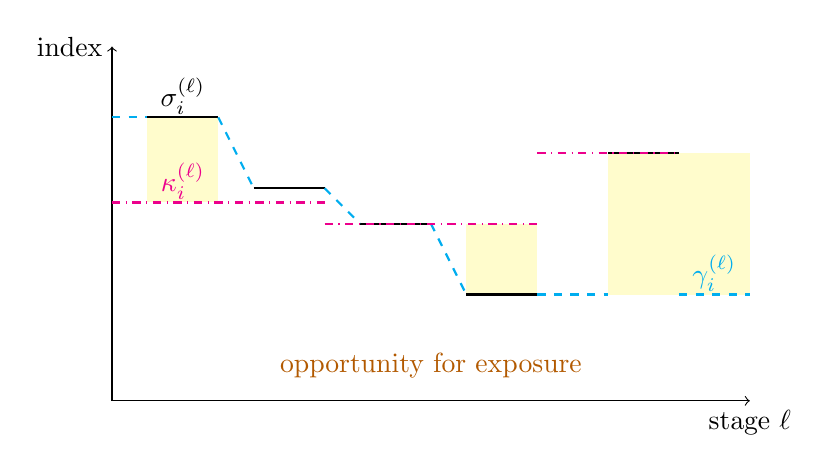
\begin{tikzpicture}[scale=0.9]
    % Define coordinates and dimensions
    \def\xmax{9}
    \def\ymax{5}
    
    % Draw axes
    \draw[->] (0,0) -- (\xmax,0) node[below] {stage $\ell$};
    \draw[->] (0,0) -- (0,\ymax) node[left] {index};
    
    % Draw the sigma values (black solid line)
    \draw[thick] (0.5,4) -- (1.5,4);
    \draw[thick] (2,3) -- (3,3);
    \draw[thick] (3.5,2.5) -- (4.5,2.5);
    \draw[thick] (5,1.5) -- (6,1.5);
    \draw[thick] (7,3.5) -- (8,3.5);
    
    % Add sigma label
    \node at (1,4.3) {$\sigma_i^{(\ell)}$};
    
    % Draw gamma values (cyan dashed line)
    \draw[cyan, dashed, thick] (0,4) -- (0.5,4);
    \draw[cyan, dashed, thick] (1.5,4) -- (2,3);
    \draw[cyan, dashed, thick] (3,3) -- (3.5,2.5);
    \draw[cyan, dashed, thick] (4.5,2.5) -- (5,1.5);
    \draw[cyan, dashed, thick] (6,1.5) -- (7,1.5);
    \draw[cyan, dashed, thick] (8,1.5) -- (9,1.5);
    
    % Add gamma label
    \node[cyan] at (8.5,1.8) {$\gamma_i^{(\ell)}$};
    
    % Draw kappa values (magenta dash-dot line)
    \draw[magenta, dash dot, thick] (0,2.8) -- (3,2.8);
    \draw[magenta, dash dot, thick] (3,2.5) -- (6,2.5);
    \draw[magenta, dash dot, thick] (6,3.5) -- (8,3.5);
    
    % Add kappa label
    \node[magenta] at (1,3.1) {$\kappa_i^{(\ell)}$};
    
    % Add yellow background for exposure opportunity regions
    \begin{scope}[on background layer]
        \fill[yellow!20] (0.5,2.8) rectangle (1.5,4);
        \fill[yellow!20] (5,1.5) rectangle (6,2.5);
        \fill[yellow!20] (7,1.5) rectangle (8,3.5);
        \fill[yellow!20] (8,1.5) rectangle (9,3.5);
    \end{scope}
    
    % Add exposure opportunity label
    \node[orange!70!black] at (4.5,0.5) {opportunity for exposure};
    
\end{tikzpicture}

\end{document}